\subsection{Purpose}

The purpose of Task B was to use the converged numerical settings from Task A
to compare structural, energetic, and magnetic properties of Ni and NiO.  For
each solid-state case, a full cell relaxation was followed by a static
single-point calculation on the relaxed structure.  The reported energies,
magnetic moments, stresses, and lattice parameters were extracted from the
static calculations.

\subsection{Computational Setup and Assumptions}

The Task B calculations used the conservative converged settings selected after
Task A.  For Ni, the calculations used \texttt{ENCUT = 520 eV} and a
\(24\times24\times24\) Gamma-centered k-point mesh.  For NiO, the calculations
used \texttt{ENCUT = 700 eV} and a \(16\times16\times16\) Gamma-centered
k-point mesh.  These choices are consistent with the convergence requirements
for plane-wave cutoff and Brillouin-zone sampling discussed in the VASP
documentation \cite{vasp-encut,vasp-kpoints}.

Two Ni magnetic states were considered:
\begin{itemize}
  \item non-magnetic PBE, with \texttt{ISPIN = 1};
  \item ferromagnetic PBE, with \texttt{ISPIN = 2} and
  \texttt{MAGMOM = 4*0.6}.
\end{itemize}
This tests whether the calculation recovers the expected ferromagnetic ground
state of elemental Ni.

For NiO, four cases were considered:
\begin{itemize}
  \item PBE ferromagnetic;
  \item PBE AFM-II;
  \item DFT+\(U\) ferromagnetic;
  \item DFT+\(U\) AFM-II.
\end{itemize}
The AFM-II setup used opposite initial moments on the two Ni atoms,
\[
  \texttt{MAGMOM = 2.0 -2.0 2*0.0},
\]
while the ferromagnetic setup used
\[
  \texttt{MAGMOM = 2*2.0 2*0.0}.
\]
The AFM-II ordering was chosen because it is the standard low-energy magnetic
ordering for rocksalt NiO and is used in VASP's NiO magnetic-structure
tutorial \cite{vasp-nio-magnetism}.
The DFT+\(U\) calculations used the same Dudarev setup as in Task A:
\texttt{LDAUTYPE = 2}, \texttt{LDAUL = 2 -1},
\texttt{LDAUU = 7.2 0.0}, and \texttt{LDAUJ = 1.0 0.0}.  Thus the effective
correction on Ni \(3d\) orbitals was
\[
  U_{\mathrm{eff}} = U - J = 6.2~\mathrm{eV}.
\]
No Hubbard correction was applied to oxygen.  In this formulation only
\(U_{\mathrm{eff}}\) enters the correction energy, so the chosen
\texttt{LDAUU} and \texttt{LDAUJ} values should be understood as a
\(U_{\mathrm{eff}} = 6.2~\mathrm{eV}\) calculation rather than as independent
physical fitting of \(U\) and \(J\) \cite{dudarev,vasp-ldautype}.  This value is
within the range commonly used for NiO DFT+\(U\) examples and linear-response
estimates \cite{vasp-nio-magnetism,vasp-strong-corr}.

The relaxation calculations used \texttt{IBRION = 2}, \texttt{ISIF = 3},
\texttt{NSW = 120}, and \texttt{EDIFFG = -0.02 eV/A}, allowing both ionic
positions and cell shape/volume to relax.  Static calculations then used
\texttt{IBRION = -1}, \texttt{NSW = 0}, and \texttt{ISIF = 2}.  Metallic Ni
relaxations used \texttt{ISMEAR = 1} and \texttt{SIGMA = 0.10}.  The final
static calculations used \texttt{ISMEAR = -5}.  The use of smearing for metallic
relaxations avoids the known problem that the tetrahedron method can give
unreliable forces and stress in metals, while the tetrahedron method is
appropriate for final static total energies when no forces are used
\cite{vasp-ibrion,vasp-isif,vasp-ediffg,vasp-ismear}.

\subsection{Results}

\begin{table}[h]
\centering
\caption{Task B relaxed structures and total energies.}
\resizebox{\textwidth}{!}{%
\begin{tabular}{llrrrrrr}
\toprule
System & Method/order & \(a\) (\AA) & \(b\) (\AA) & \(c\) (\AA) &
\(\alpha=\beta=\gamma\) (deg) & \(E_{\mathrm{total}}\) (eV) & Pressure (kB) \\
\midrule
Ni  & PBE NM        & 3.5107 & 3.5107 & 3.5107 & 90.000 & -21.647642 & -0.416 \\
Ni  & PBE FM        & 3.5180 & 3.5180 & 3.5180 & 90.000 & -21.881317 & -0.453 \\
NiO & PBE FM        & 5.1576 & 5.1576 & 5.1576 & 33.560 & -22.966480 &  3.354 \\
NiO & PBE AFM-II    & 5.1281 & 5.1281 & 5.1281 & 33.620 & -23.495908 & -3.010 \\
NiO & DFT+\(U\) FM     & 5.1383 & 5.1383 & 5.1383 & 33.557 & -20.343218 & -0.041 \\
NiO & DFT+\(U\) AFM-II & 5.1194 & 5.1194 & 5.1194 & 33.568 & -20.490702 & -0.016 \\
\bottomrule
\end{tabular}%
}
\end{table}

In VASP's stress convention, positive diagonal stress corresponds to positive
\texttt{external pressure}, while negative diagonal stress corresponds to
negative \texttt{external pressure}; equivalently, positive diagonal stress
indicates a compressive state that tends to expand the cell, and negative
diagonal stress indicates a tensile state that tends to reduce the cell volume
\cite{vasp-isif}.  The PBE NiO ferromagnetic static calculation therefore has
a small compressive residual pressure (about
\(3.35~\mathrm{kB}=0.335~\mathrm{GPa}\)), while the PBE AFM-II static
calculation has a small tensile residual pressure (about
\(-3.01~\mathrm{kB}=-0.301~\mathrm{GPa}\)).  These residual stresses are minor
compared with the elastic constants of NiO and arise after doing a final static
single-point calculation with tetrahedron integration on the relaxed geometry.
The much smaller residual pressures in the DFT+\(U\) NiO cases show that the
final DFT+\(U\) geometries are closer to the zero-stress condition under the
corresponding static settings.

\begin{table}[h]
\centering
\caption{Task B magnetic moments and cohesive energies.}
\resizebox{\textwidth}{!}{%
\begin{tabular}{llrll}
\toprule
System & Method/order & Total moment (\(\mu_B\)) & Local moments (\(\mu_B\)) & Cohesive energy (eV) \\
\midrule
Ni  & PBE NM        & --      & --                         & 4.778453 \\
Ni  & PBE FM        & 2.5040  & 0.638, 0.638, 0.638, 0.638 & 4.836872 \\
NiO & PBE FM        & 3.6109  & 1.479, 1.479, 0.280, 0.280 & 9.303126 \\
NiO & PBE AFM-II    & 0.0000  & 1.350, -1.350, 0.000, 0.000 & 9.567840 \\
NiO & DFT+\(U\) FM     & 4.0000  & 1.825, 1.825, 0.169, 0.169 & 7.991495 \\
NiO & DFT+\(U\) AFM-II & 0.0000  & 1.748, -1.748, 0.000, 0.000 & 8.065237 \\
\bottomrule
\end{tabular}%
}
\end{table}

\begin{table}[h]
\centering
\caption{Task B residual forces and final static stress tensors.  Stresses are
reported in VASP order \(xx, yy, zz, xy, yz, zx\), in kB.}
\resizebox{\textwidth}{!}{%
\begin{tabular}{llrl}
\toprule
System & Method/order & Max force (eV/\AA) & Stress tensor (kB) \\
\midrule
Ni  & PBE NM        & 0.0000 & \(-0.42, -0.42, -0.42, 0.00, -0.00, 0.00\) \\
Ni  & PBE FM        & 0.0000 & \(-0.45, -0.45, -0.45, 0.00, 0.00, 0.00\) \\
NiO & PBE FM        & 0.0000 & \(3.35, 3.35, 3.35, 0.04, 0.04, 0.04\) \\
NiO & PBE AFM-II    & 0.0000 & \(-3.01, -3.01, -3.01, -1.64, -1.64, -1.64\) \\
NiO & DFT+\(U\) FM     & 0.0000 & \(-0.04, -0.04, -0.04, 0.00, 0.00, 0.00\) \\
NiO & DFT+\(U\) AFM-II & 0.0000 & \(-0.02, -0.02, -0.02, -0.45, -0.45, -0.45\) \\
\bottomrule
\end{tabular}%
}
\end{table}

\begin{figure}[htbp]
\centering
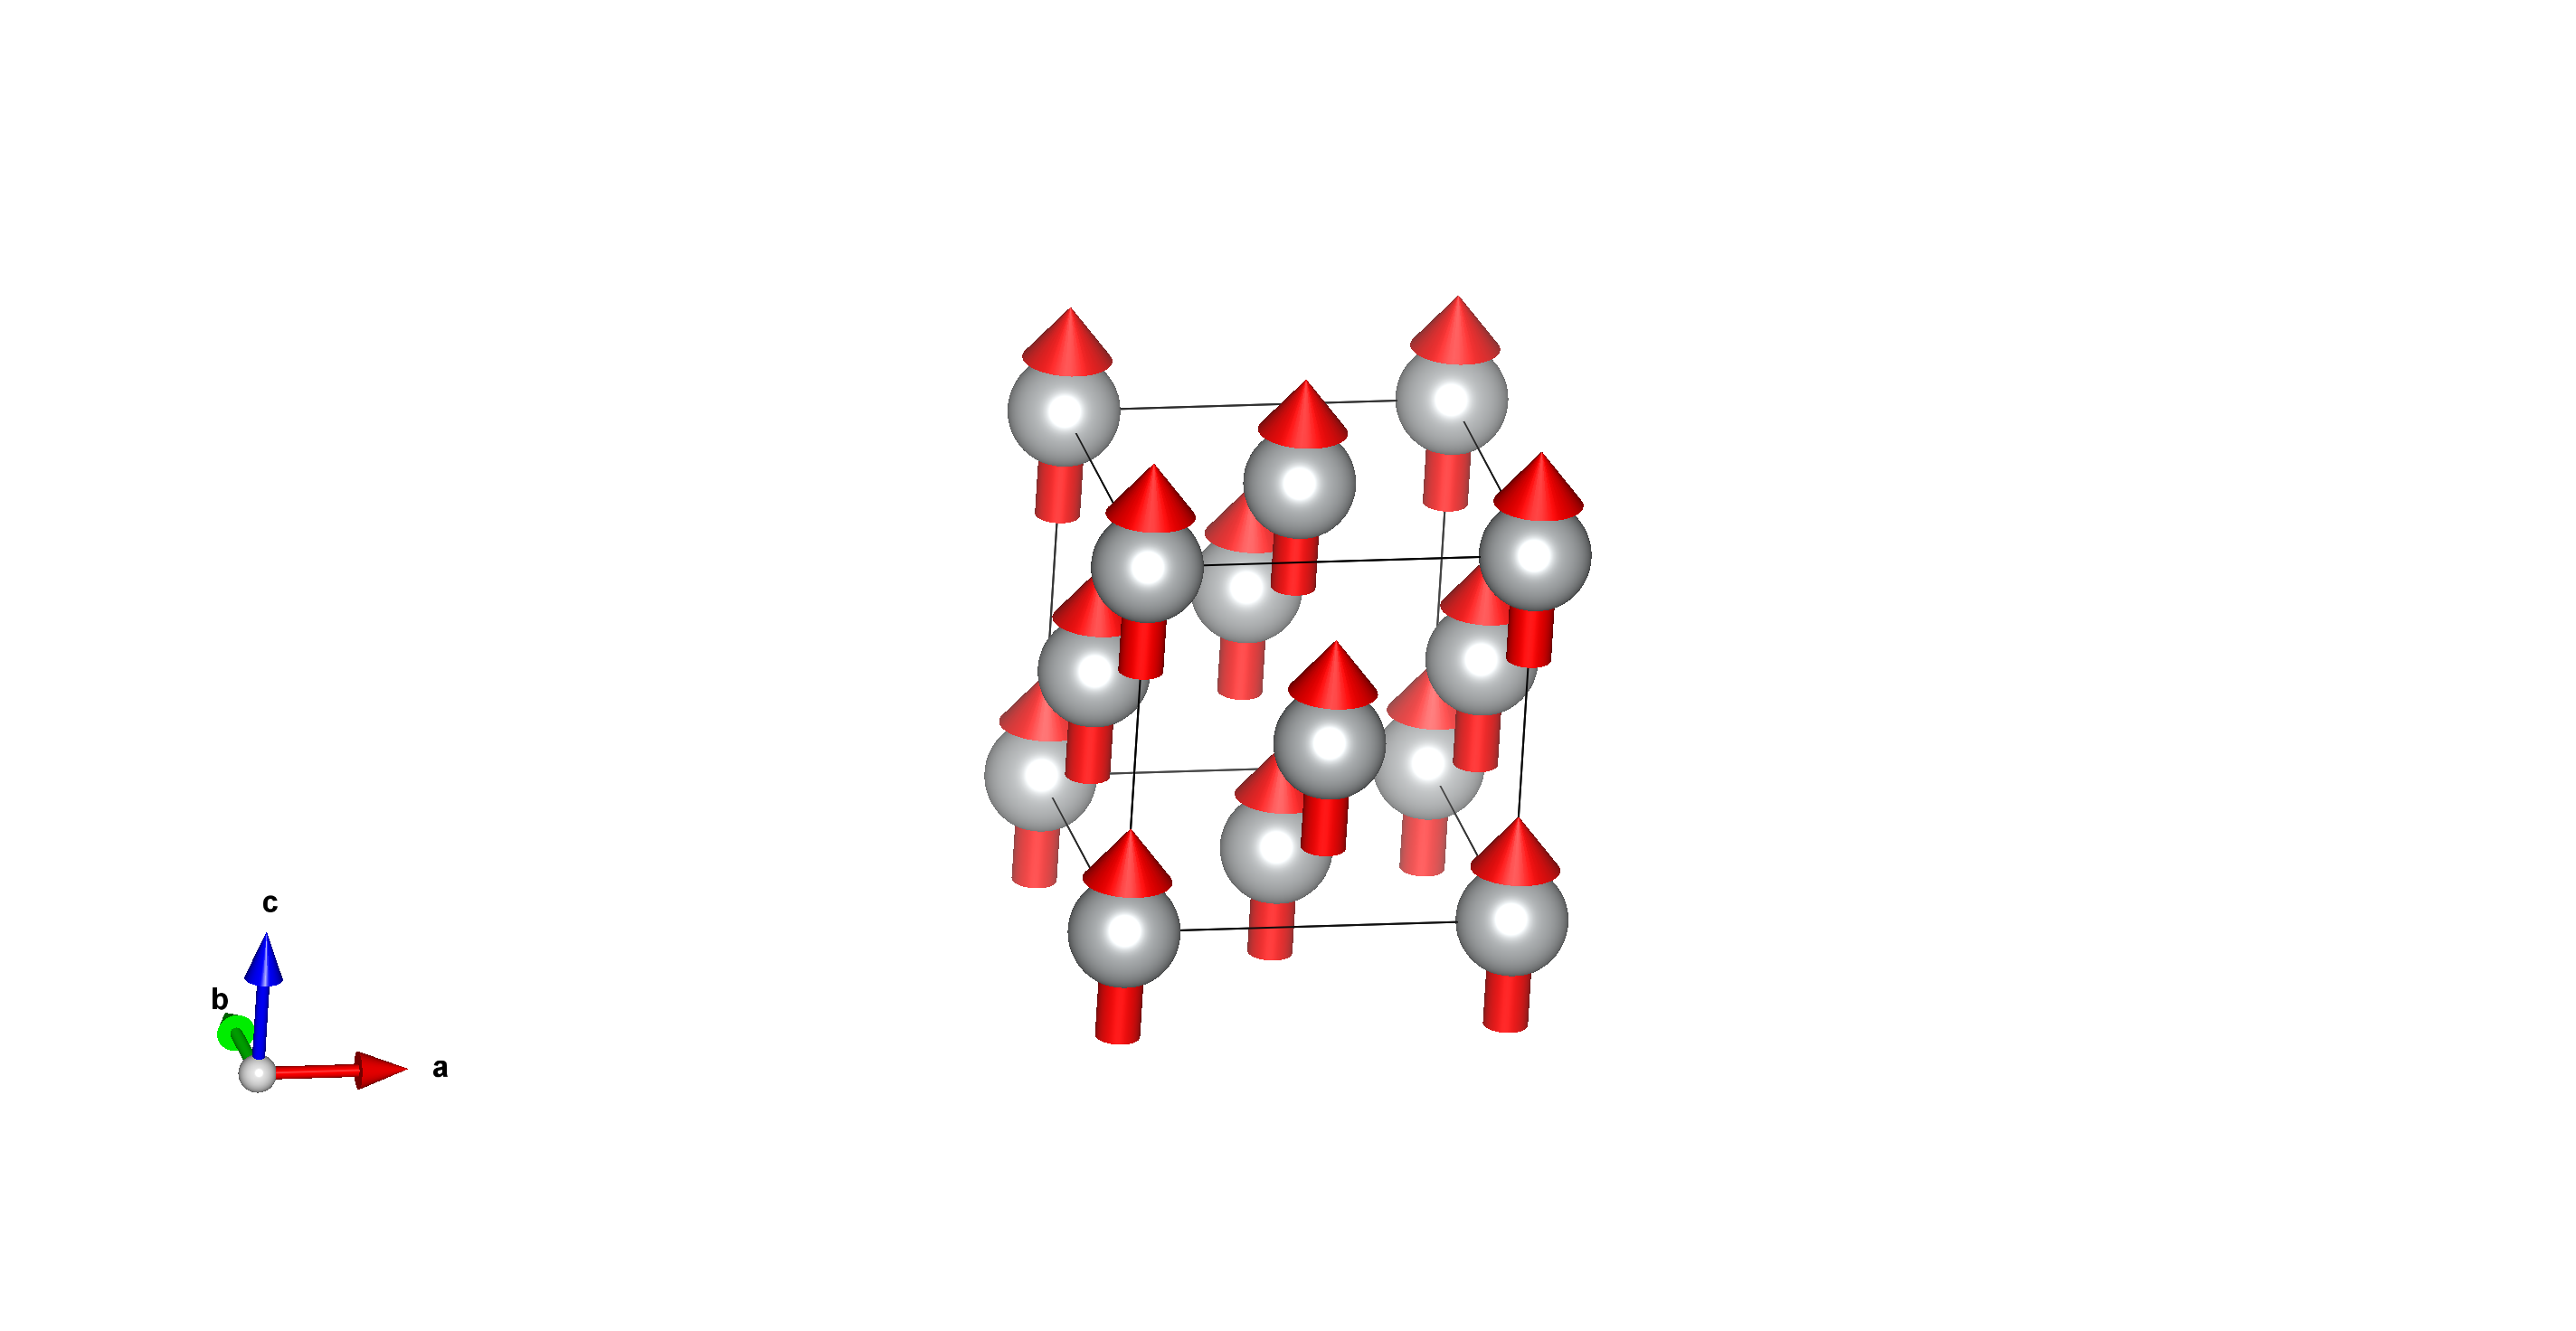
\includegraphics[width=0.9\textwidth]{figures/Ni_relaxed_FM_structure.png}
\caption{Relaxed ferromagnetic fcc Ni structure used in the final PBE static
calculation.  The arrows indicate parallel Ni magnetic moments.}
\label{fig:task-b-ni-fm-structure}
\end{figure}

\begin{figure}[htbp]
\centering
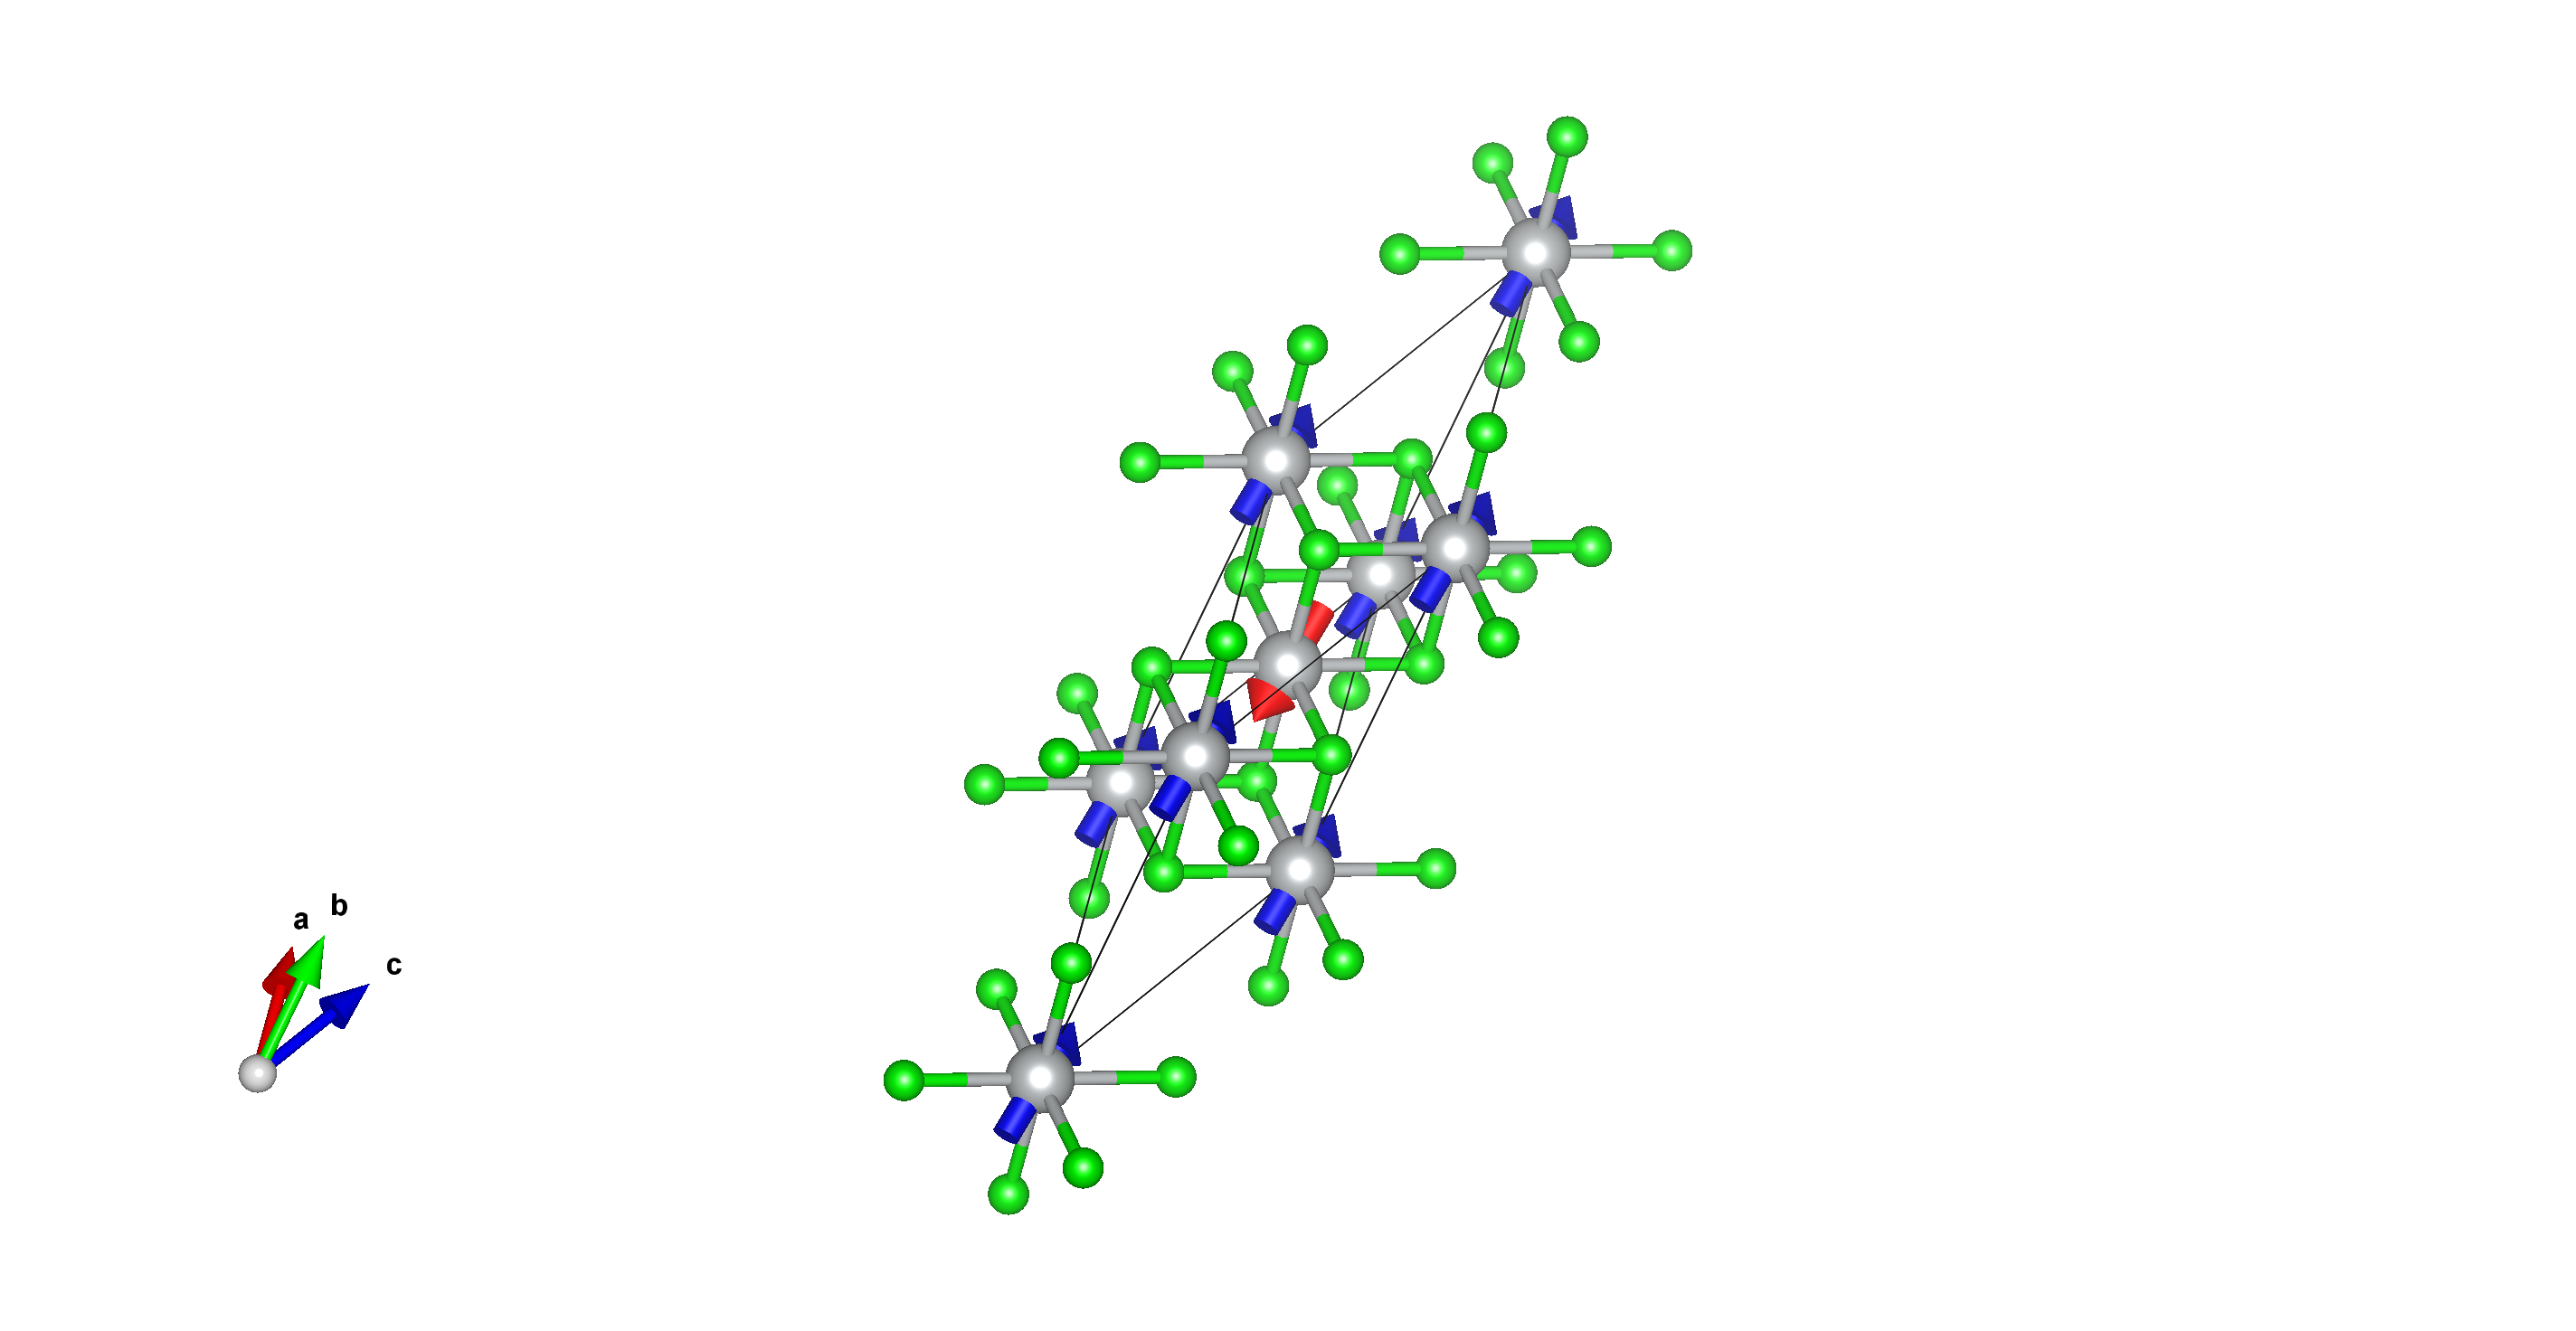
\includegraphics[width=0.9\textwidth]{figures/NiO_relaxed_AFM_structure.png}
\caption{Relaxed rocksalt NiO structure in the DFT+\(U\) AFM-II magnetic
ordering.  The arrows indicate antiparallel Ni magnetic moments on alternating
planes; O atoms carry no assigned spin moment.}
\label{fig:task-b-nio-afm-structure}
\end{figure}

The Ni results show that the ferromagnetic state is lower in energy than the
non-magnetic state by
\[
  -21.881317 - (-21.647642) = -0.233675~\mathrm{eV}
\]
per four-atom cell, or approximately \(58.4~\mathrm{meV}\) per Ni atom.  This
confirms that the ferromagnetic phase is the stable magnetic solution among the
two Ni states tested here.

For NiO, AFM-II is lower in energy than the ferromagnetic state for both PBE
and DFT+\(U\).  In PBE, the energy lowering is
\[
  -23.495908 - (-22.966480) = -0.529428~\mathrm{eV}
\]
per two-NiO cell, or \(264.7~\mathrm{meV}\) per NiO formula unit.  With
DFT+\(U\), the energy lowering is
\[
  -20.490702 - (-20.343218) = -0.147484~\mathrm{eV}
\]
per two-NiO cell, or \(73.7~\mathrm{meV}\) per NiO formula unit.  Therefore,
among the magnetic states tested in this project, AFM-II is the most stable
ordering of NiO.

\subsection{Cohesive Energy}

The cohesive energy was evaluated as
\[
  E_{\mathrm{coh}} =
  \frac{n_{\mathrm{Ni}}E_{\mathrm{Ni,atom}} +
        n_{\mathrm{O}}E_{\mathrm{O,atom}} -
        E_{\mathrm{solid}}}{n_{\mathrm{Ni}}},
\]
where the denominator is the number of Ni atoms.  For pure Ni this is the usual
cohesive energy per Ni atom.  For NiO, this denominator is also the number of
NiO formula units in the AFM-II cell, so the values are cohesive energies per
NiO formula unit.  The isolated Ni and O reference calculations both completed
successfully using single-element PAW datasets.  The ferromagnetic Ni cohesive energy is
\(4.836872~\mathrm{eV}\), slightly larger than the non-magnetic value
\(4.778453~\mathrm{eV}\), consistent with ferromagnetic Ni being more stable.
For the lowest-energy NiO case, DFT+\(U\) AFM-II, the cohesive energy is
\(8.065237~\mathrm{eV}\) per NiO formula unit.

The cohesive energies should be interpreted as internally consistent
same-method quantities rather than as direct experimental heats of formation.
They depend on the isolated-atom reference energies, spin states, PAW datasets,
and on whether the DFT+\(U\) correction is applied.  This is why the PBE and
DFT+\(U\) NiO cohesive energies are not meant to be compared as absolute
thermochemical predictions across methods.  Within each method, however, the
values have the expected sign and scale: the solids are bound relative to the
separated atoms, and the magnetic ground-state choices give the larger
cohesive energies.

\subsection{Discussion}

The Task B results are physically consistent.  Elemental Ni relaxes to a
ferromagnetic solution with a finite moment of about \(0.638~\mu_B\) per atom.
The energy lowering of \(58.4~\mathrm{meV}\) per atom relative to the
non-magnetic state is not large on the scale of chemical bond energies, but it
is large compared with the numerical convergence target from Task A.  The
magnetic stabilization is therefore a real result of the calculation rather
than a cutoff or k-point artifact.  The small increase of the relaxed lattice
parameter from the non-magnetic to the ferromagnetic solution is also
reasonable, because spin polarization changes the balance between exchange
splitting, band filling, and bonding in the partly occupied Ni \(d\) bands.

For NiO, the AFM-II states have nearly zero total magnetic moment because the
two Ni local moments cancel.  The DFT+\(U\) AFM-II calculation gives larger
local Ni moments, about \(1.748~\mu_B\), than the PBE AFM-II calculation,
about \(1.350~\mu_B\).  This is expected because the Hubbard correction
localizes the Ni \(3d\) electrons more strongly.  The same localization also
reduces the energy difference between the ferromagnetic and AFM-II NiO states
from \(264.7~\mathrm{meV}\) per formula unit in PBE to
\(73.7~\mathrm{meV}\) per formula unit in DFT+\(U\).  This does not change the
qualitative conclusion: for both electronic-structure descriptions the
AFM-II ordering remains the lowest of the magnetic states tested here.

The comparison with literature values is also reasonable.  The relaxed Ni
lattice parameter, \(a = 3.518~\mathrm{\AA}\), and the moment
\(0.638~\mu_B\) per atom are close to the standard ferromagnetic fcc Ni values
used in VASP benchmark examples \cite{vasp-fcc-ni}.  For NiO, the AFM-II
ordering is the expected magnetic ground state for rocksalt NiO
\cite{vasp-nio-magnetism}.  The DFT+\(U\) AFM-II local moment of
\(1.748~\mu_B\) per Ni is larger than the PBE value and lies in the physically
expected range for localized Ni \(3d\) moments in NiO; the use of a Dudarev
Hubbard correction and the resulting enhancement of the Ni moment are
consistent with the LSDA+\(U\) analysis of Dudarev \emph{et al.}
\cite{dudarev}.  The relaxed AFM-II NiO cell has a rhombohedral magnetic-cell
vector length of \(5.119~\mathrm{\AA}\), corresponding to an underlying
rocksalt cubic lattice parameter of about \(4.18~\mathrm{\AA}\), close to the
starting Materials Project rocksalt NiO structure and typical experimental
values for bulk NiO \cite{mp-nio,dudarev}.

The residual stresses are also compatible with well-relaxed structures.  The
largest pressure magnitude in the final static calculations is only about
\(3.35~\mathrm{kB}\), or \(0.335~\mathrm{GPa}\), much smaller than the elastic
moduli obtained in Task E.  The opposite pressure signs for PBE FM and PBE
AFM-II NiO therefore should not be read as a qualitative contradiction; they
mainly indicate that the final tetrahedron static calculation samples a
slightly different stress point than the relaxation step, and that the two
magnetic states prefer slightly different equilibrium volumes.
